\documentclass[11pt,a4paper]{article}

\usepackage[left=2cm,text={17cm,24cm},top=3cm]{geometry}
\usepackage[bookmarksopen,colorlinks,plainpages=false,urlcolor=blue,unicode,linkcolor=blue]{hyperref}
\usepackage[czech]{babel}
\usepackage[utf8]{inputenc}
\usepackage[T1]{fontenc}
\usepackage{indentfirst}
\usepackage{graphicx}
\usepackage{enumitem}
\usepackage{float}
\usepackage{url}

\graphicspath{{.}}

\begin{document}

% #################################################################################################
% TITLEPAGE

\begin{titlepage}
    \begin{center}
        \Huge
        \textsc{
            Fakulta informačních technologií\\
            Vysoké učení technické v~Brně
        }
        \vspace{100px}
        \begin{figure}[!h]
            \centering
            
\includegraphics[scale=0.7]{img/vutfitlogo.png}
        \end{figure}
        \\[20mm]
        \huge{
            \textbf{
                IMP \,--\, Mikroprocesorové a vestavěné systémy
            }
        }
        \\[2em]
        \LARGE{
            \textbf{
                Hodiny s~budíkem na bázi modulu \\ Real Time Clock (RTC)
            }
        }
        \vfill
    \end{center}
        \Large{
            Adam Dalibor Jurčík (xjurci08) \hfill \today
        }

\end{titlepage}

% #################################################################################################
% CONTENT

\setlength{\parskip}{0pt}
\hypersetup{hidelinks}
\tableofcontents
\setlength{\parskip}{0pt}

\newpage %#########################################################################################

\section{Úvod}
Zadáním je vytvořit hodiny s~budík s~modulem Real Time Clock. Dále má splňovat určité uživatelské funkce:

\begin{itemize}
        \item nastavení času
        \item ovládání budíku (zapnutí, vypnutí)
        \item nastavení času alarmu
        \item nastavení zvukové signalizace z~alespoň tří typů
        \item nastavení světelné signalizace z~alespoň tří typů
        \item nastavení opakování alarmu, z~čehož vyplývá nastavení času, po kterém se bude opakovat
    \end{itemize}

Hardware budíku je Minerva 1 (Fitkit3) a ovládat se bude dát pomocí aplikace \emph{PuTTY} na softwaru Windows 10.

\section{Spuštění}
Hardware připojíte pomocí drátu tiskárny a ve \emph{Správci zařízení} si najdete část s~\emph{porty}, kde se dočtete jakou má zkratku kde x představuje číslo (\verb|COMx|). Dále pro nahrání implementace budete potřebovat programovací aplikaci \emph{Kinetis}, díky které spustíte zařízení. Dále je potřeba zapnout komunikaci přes \emph{PuTTY}. To uděláte přepnutí na \emph{serial} komunikaci, kde vyberete vaše zařízení (předešlý krok kde jste zjistili zkratku) a rychlost změníte na 115200 baudů.

\subsection{Nastavení času}
Hned po spuštění vám budík nabídne nastavení času. Dané datum musí být zadané na jednou, jestli se překliknete a něco smažete nebo se budete snažit posunout se šipkami na klávesnici, datum se neuloží, ale budete jej moci zadat znovu.

\section{Ovládání}
V~aplikaci \emph{PuTTY} se uživateli ukazují dotazy a on je schopen na ně odpovědět a zařízení se podle jeho příkazů naprogramuje. Pokud uživatel napíše špatný příkaz, je mu nabídnuto se opravit. Se zařízením lze komunikovat pouze přes počítač, takže musí být stále připojeno.

\subsection{Nastavení zvukové signalizace}
Uživatel je schopen přes aplikaci \emph{PuTTY} dokáže nastavit a vyzkoušet 3 typy zvukové signalizace. Výběr i vyzkoušení se provede po zadání příkazu, když je uživatel vyzván. Pro vyzkoušení signalizace je potřeba napsat do \emph{Inputu} \verb|try|\textbf{X}, kde \textbf{X} je číslo signalizace. Výběr se pak udělá pomocí zadání čísla.

\subsection{Nastavení světelné signalizace}
Tato signalizace se provádí na diodách, které se nachází vedle tlačítek na zařízení. Stejně tak u~zvukové signalizace dokáže uživatel pomocí stejných příkazů vybrat nebo vyzkoušet ze tří typů signalizace.

\subsection{Nastavení opakování}
Opakování lze nastavit od 0 až po 5. Nula opakování znamená, že budík spustí obě signalizace a skončí. Každé další číslo přidá jedno k~tomu, co zvoní přesně na zvolený čas. Realita je tedy taková, že pokud uživatel zvolí 5 opakování budík bude zvonit 6x s~přestávkami.

\subsubsection{Nastavení času opakování}
Pokud uživatel zvolí nastavení opakování na 1-5, tak je vyzván, aby zadal dobu, po které se budík bude opakovat. Nejmenší doba opakování je 30 sekund a maximální je 300 sekund, což je 5 minut.

\subsection{Nastavení času alarmu}
Po vybrání všech potřebných věcí pro funkčnost budíku, je uživatel vyzván aby zadal čas, kdy má být budík spuštěn. Stejně tak jako u~nastavení času je potřeba neudělat chybu, ale pokud se tak stane můžete ho zadat znovu.

\subsection{Budík v~pohotovosti}
Když je budík zapnut, lze mu dávat příkazy. Jedná se třeba o~příkaz aby se vypnul - \verb|turnoff|. Budík po něm úplně vypne. Dále je možné použít příkaz pro restart - \verb|restart|. Pokud uživatel chce vypnout buzení neboli signalizaci, že nastal čas, který zvolil tak použije příkaz \verb|alarmoff|. To se ukáže tak, že budík v~aktivním stavu neukazuje nastavený čas signalizace, ale slovo \verb|OFF|. Samozřejmě uživatel dokáže nastavit nový čas signalizace příkazem - \verb|newalarm|, který však přepíše dříve nastavený čas, pokud takový nějaký je. Dalším příkazem je \verb|help|, kdy se pouze vypíše, co jednotlivé příkazy provádí.

Pokud je nastaven budík a nadejde čas zadaný uživatelem pro signalizaci, spustí se sekvence pípání a následně blikání. Signalizace skončí sama, uživatel ji nemusí vypínat. Po skončení budík vyzve uživatele k~zadání příkazu, neboli je ve \emph{standby} režimu.

\section{Implementace}
Pro implementaci byli využity zkušenosti hlavně ze cvik a jejich zdrojové kódy. Implementace se nachází v~souboru \verb|main.c|. Zdrojový kód je rozdělen do několika částí: globální proměnné, jednoduché funkce (například pípání), funkce pro načtení času od uživatele, inicializace, signalizace, \emph{RTC modul} a funkce \emph{main}, která obsahuje implementaci konečného automatu.

\subsection{Inicializace}
Na začátku funkce \emph{main} se inicializuje \emph{MCU}, porty, \emph{UART5}, a \emph{RTC modul}. Definují se lokální proměnné a vstoupí se do nekonečného \emph{whilu}. V~této funkci se nachází zmiňovaný konečný automat, podle kterého se budík řídí. V~každém stavu se pracuje se vstupem (proměnná \verb|input|), který je načten a určí se co se má provést a následně pokračovat dále třeba do dalšího stavu. Proměnné s~předponou \verb|sec_| jsou typu \emph{unsigned int}, jelikož nesou registry \emph{RTC modulu} a ty jsou velké 32 bitů.

\subsection{Signalizace alarmu}
Signalizace probíhá způsobem, že budík prvně zvoní a pak bliká vybranými signalizacemi. To provádí funkce \verb|RTC_IRQHandler|, která zavolá funkce \verb|Play_song| a \verb|LED_on|, kdy u~obou je parametr globální proměnná s~hodnotou zvuku a světla, kterou si vybral uživatel. Nachází se tam taky implementace odložení, když po každém zazvonění budík dekrementuje globální proměnnou s~hodnotou kolikrát se má opakovat.

\subsection{FSM}
V~kódu se střídá osm stavů, kdy \emph{START} je počáteční stav a \emph{END} konečný. Uživatel je schopen zadávat příkazy pro ovládání budíku jen ve stavu \emph{ON}, kde je budík aktivovaný. Pro nastavení budíku se program přesune do stavu \emph{SONG}, uživatel může vyzkoušet přednastavené pípání. Poté pokračuje v~nastavení do zbylých stavů. Při příkazu \verb|restat|, je uživatel dotázán jaký chce nastavit čas a po úspěšném nastavené se přesune zpět do pohotovosti. Po příkazu \verb|turnoff| se program přesune do stavu \emph{END}, kde se spustí vypnutí budíku.
\begin{figure}[!h]
    \centering
    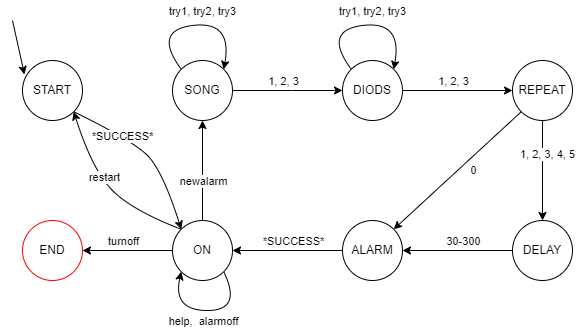
\includegraphics[scale=0.6]{img/FSM.png}
    \caption{Konečný automat}
\end{figure}

\subsection{RTC modul}
Modul používá 32 bitové číslo a tak se čas zadaný uživatelem převádí do sekund a pro zobrazení v~\emph{PuTTY} se převádí zase zpět na formát \verb|YYYY-MM-DD HH:MM:SS|, to vykonávají funkce \verb|Input_time| a \verb|convert| pomocí funkce \verb|strftime| z~knihovny \verb|time.h|. Do proměnné je uložen počet sekund od epochy 1.1.1970 až do čas, který byl zadaný uživatelem.

\verb|RTC_IRQHandler| obsluhuje přerušení od \emph{RTC} ve které je implementovaná signalizace budíku a její od opakování.

\section{Bodování}
\begin{itemize}
        \item E -- 0,9b
        \item F -- 5b
        \item P -- 0,9b
        \item Q -- 0,9b + 1b + 0,9b
        \item D -- 0,8b + 1,9b + 0,9b
        \item (0,25 + 0,75 * 5/5) * (0,9 + 5 + 2,8 + 0,9 + 3,6) = 13,2b
    \end{itemize}


\end{document} %###################################################################################